\documentclass[12pt]{article}

\usepackage[X2,T2A]{fontenc}
\usepackage[utf8]{inputenc}
\usepackage[russian]{babel}
\usepackage[a4paper, margin=1in]{geometry}
\usepackage{graphicx}
\usepackage{amsmath}
\usepackage{wrapfig}
\usepackage{multirow}
\usepackage{mathtools}
\usepackage{pgfplots}
\usepackage{pgfplotstable}
\usepackage{setspace}
\usepackage{changepage}
\usepackage{caption}
\usepackage{csquotes}
\usepackage{hyperref}
\usepackage{listings}


\pgfplotsset{compat=1.18}
\hypersetup{
  colorlinks = true,
  linkcolor  = blue,
  filecolor  = magenta,      
  urlcolor   = darkgray,
  pdftitle   = spec-storage-het,
}

\begin{document}

\begin{titlepage}
  \begin{center}
    \begin{spacing}{1.4}
      \large{Университет ИТМО} \\
      \large{Факультет программной инженерии и компьютерной техники} \\
    \end{spacing}
    \vfill
    \textbf{
      \huge{Описание сервиса.} \\
      \huge{Сеть хранилищ} \\
    }
  \end{center}
  \vfill
  \begin{center}
    \begin{tabular}{r l}
      Смирнов Виктор Игоревич  & P32131 \\
    \end{tabular}
  \end{center}
  \vfill
  \begin{center}
    \begin{large}
      2023
    \end{large}
  \end{center}
\end{titlepage}

\tableofcontents

\section{Введение}

\subsection{Задача}
Выбрать любую реально существующую систему и 
описать её в терминах UML. Желательно, чтобы 
система была не полностью информационной, но 
опиралась на информационную систему как 
показано в примере на лекции (Point of sale). 
Необходимо описать границы системы на разных 
уровнях, а также описать сценарии использования 
для нескольких Акторов.


Отчёт по работе должен содержать:
\begin{enumerate}
  \item Титульный лист с указанием автора и номера группы
  \item Само задание
  \item Описание рассматриваемой системы с требованиями к ней
  \item Формальное описание системы с необходимым количеством UML диаграмм
  \item Словесное описание сценариев сценариев использование для рассматриваемых акторов
\end{enumerate}


\subsection{О документе}
Документ представляет из себя описание
системы "Система хранилищ" и требований к ней.
Документ содержит:

\begin{enumerate}
  \item Описание рассматриваемой системы с требованиями к ней
  \item Формальное описание системы с необходимым количеством
        UML диаграмм
  \item Словесное описание сценариев сценариев использование
        для рассматриваемых акторов
\end{enumerate}


\subsection{Описание системы}
Сервис должен давать возможность управлять
хранилищем и перевозками: получать список хранимых 
вещей в любой момент времени, добавлять/удалять вещи в 
данном хранилище, добавлять/удалять ячейки в данном хранилище,
вести учет перевозок вещей из одного склада в другой, 
хранить историю действий с хранимыми сущностями,
отслеживать путь конкретного заказа через всю сеть хранилищ,
поддерживать разграничение доступа к хранимым данным.


\subsection{Ключевые слова и их синонимы}
\begin{enumerate}
  \item \textbf{Хранилище} - склад, контейнер, содержит предметы

  \item \textbf{Предмет} - товар, вещь, продукт

  \item \textbf{Администраторы хранилища $A$, Администратор} - группа физических
        лиц, управляющее заданным хранилищем $A$

  \item \textbf{Менеджер сети хранилищ $A$, Менеджер} - юридическое лицо,
        управляющее сетью хранилищ $A$, то есть множеством
        складов $A_1, A_2, ..., A_n$

  \item \textbf{Перевозчик} - юридическое лицо, представляющее
        услуги логистики, в нашем сервисе осуществляющее перевозку
        предметов между складами

  \item \textbf{Заморозка предмета} - бронирование, запрет на 
        совершение действий с заданной сущностью системы на
        протяжении заданного периода времени.

  \item \textbf{Исток, поставщик} - юридическое лицо, 
        осуществляющее поставку предметов в сеть хранилищ.

  \item \textbf{Сток, заказчик} - юридическое лицо,
        забирающее предметы из сети хранилищ, по сути покупатель
        товаров либо их распределитель.
\end{enumerate}

\section{Общее описание}

\subsection{Решаемая проблема}
Проблемы и задачи, решаемые данной системой:

\begin{enumerate}
  \item Учет предметов на хранилищах.
  
  \item Получения состояние хранилища в любой момент времени.
  
  \item Генерация отчетов по операциям с хранилищем по заданному
        промежутку времени.
        
  \item Учитывая длительные перевозки предметов между хранилищами
        в сети, прогнозирование состояния хранилища в заданный 
        момент времени.

  \item Заморозка предметов в хранилище для временной блокировки 
        операций их перемещения в сети.
      
  \item Планироваие перемещений предметов между хранилищами.
  
  \item Объединение предметов в заказы, для отслеживания операций 
        с ними.

  \item Получение историю по всем операциям в рамках одного заказа.
  
  \item Гарантия неотрицательности баланса любого предмета в
        любом хранилище сети

  \item Учет срока годности предметов.
\end{enumerate}

\subsection{Функционал продукта}
Сервис должен давать возможность управлять
хранилищем и перевозками: получать список хранимых 
вещей в любой момент времени, добавлять/удалять вещи в 
данном хранилище, добавлять/удалять ячейки в данном хранилище,
вести учет перевозок вещей из одного склада в другой, 
хранить историю действий с хранимыми сущностями,
отслеживать путь конкретного заказа через всю сеть хранилищ,
поддерживать разграничение доступа к хранимым данным.


\subsection{Описание пользователей}
\subsubsection{Администратор хранилища А}
\begin{enumerate}
  \item Распоряжается складом А
  
  \item Должен подтвержать факт прибытия вещей 
        из из склада $A_i$ в какой-то склад $A_j$, 
        где $A_i, A_j \in A$

  \item Должен подтвержать запросы на 
        перевозку вещей из склада $A_i$
        в какой-то склад $A_j$, где $A_i, A_j \in A$

  \item Может выполнять операции по 
        трансформации ячеек в складе А
\end{enumerate}


\subsubsection{Менеджер сети хранилищ А}
\begin{enumerate}
  \item Может создавать запросы на перевозку
        товаров из склада $A_i \in A$ в склад $A_j \in A$

  \item Инициирует сбор заказа в сети хранилищ A
  
  \item Может отменять действия в сети хранилищ А,
        путем инициации обратных процессов
\end{enumerate}


\section{Функциональные требования}
\begin{enumerate}
  \item Система должна вести учет предметов 
        в сети хранилищ
        
  \item Система должна предоставлять доступ к
        списку предметов в заданном хранилище

  \item Система должна предоставлять доступ к
        списку предметов во всей сети хранилищ

  \item Система должна должна предоставлять
        историю операций с заданным хранилище,
        во всей сети, по заданному заказу

  \item Система должна учитывать перемещения
        предметов между складами, предоставляя
        доступ к актуальным данным в заданный
        момент времени в том числе прошедший

  \item Система должна, опираясь на информацию
        о перемещениях предметов, предсказывать
        состояние системы в будущий момент времени

  \item Система должна гарантировать неотрицательный
        баланс по каждому предмету в каждом хранилище
        сети

  \item Система должна гененировать переодические 
        отчеты по состоянию сети и своим операциям

\end{enumerate}

\section{Сценарии использования}
\subsection{Инициация поставки в хранилище}

\textbf{Участники:}
Менеджер, Администратор, Поставщик.

\textbf{Описание:}
Менеджер договаривается с Поставщиком о
поставке предметов в хранилище. Далее Менеджер 
создает в Системе заявку на поставку предметов в 
хранилище А. Администратор хранилища либо подтверждает 
заявку на поставку предметов, либо отклоняет ее. В 
любом процесс прекращается уведомлением Менеджера и 
поставщика.

\begin{figure}[h]
  \centering
  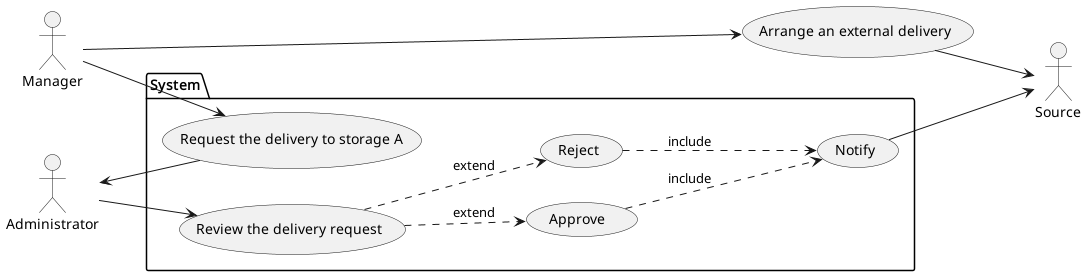
\includegraphics[width=12cm]{../../out/spec/figure/usecase/delivery_arrange/Storage Net, Use Case, Delivery Arrange.png}
  \caption{Use Case: Delivery Arrange}
\end{figure}


\subsection{Принятие поставки предметов в хранилище}

\textbf{Участники:}
Администратор.

\textbf{Описание:}
Админимтратор ожидает прибытия предметов, после 
чего подтвержает прибытие предметов в хранилище.

\begin{figure}[h]
  \centering
  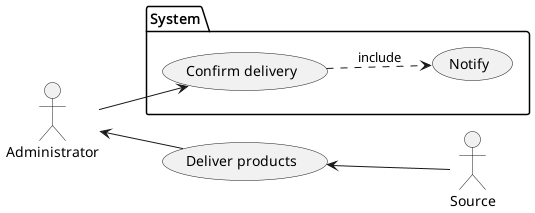
\includegraphics[width=12cm]{../../out/spec/figure/usecase/delivery_confirm/Storage Net, Use Case, Delivery Confirm.png}
  \caption{Use Case: Delivery Confirm}
\end{figure}


\subsection{Инициации перемещения предметов между хранилищами}

\textbf{Участники:}
Менеджер, Администратор, Перевозчик.

\textbf{Описание:}
Менеджер договаривается с Перевозчиком о перевозке груза из 
хранилища А в хранилище Б. Менеджер создает заявку на перемещение
предметов из хранилища А в хранилище Б. Администраторы хранилищ 
А и Б подтверждают либо отклоняют ее.

\begin{figure}[h]
  \centering
  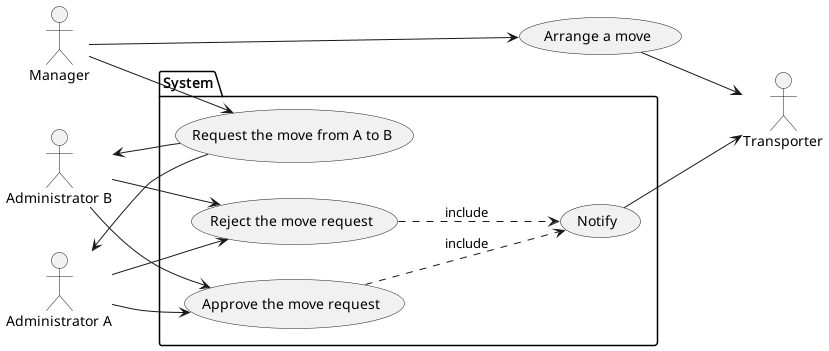
\includegraphics[width=12cm]{../../out/spec/figure/usecase/move_arrange/Storage Net, Use Case, Move Arrange.png}
  \caption{Use Case: Move Arrange}
\end{figure}

\subsection{Отправление предметов из хранилище}
Аналогично прибытию товаров в хранилище, но наоборот.

\begin{figure}[h]
  \centering
  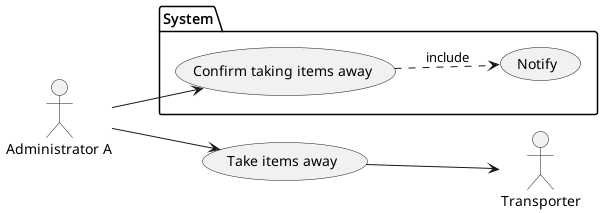
\includegraphics[width=12cm]{../../out/spec/figure/usecase/move_from_confirm/Storage Net, Use Case, Move from begin.png}
  \caption{Use Case: Move from begin}
\end{figure}

\subsection{Прибытие предметов в хранилище}
Аналогично поставке товаров в хранилище, но с перевозчиком.


\subsection{Изъятие предметов из сети хранилищ}

\textbf{Участники:}
Менеджер, Администратор, Заказчик.

\textbf{Описание:}
Заказчик договаривается с Менеджер об
изъятии предметов из конечного хранилища. Далее Менеджер 
создает в Системе заявку на изъятие предметов из 
хранилища А. Администратор хранилища либо подтверждает 
заявку на поставку предметов, либо отклоняет ее. В 
любом процесс прекращается уведомлением Менеджера и 
поставщика.

\begin{figure}[h]
  \centering
  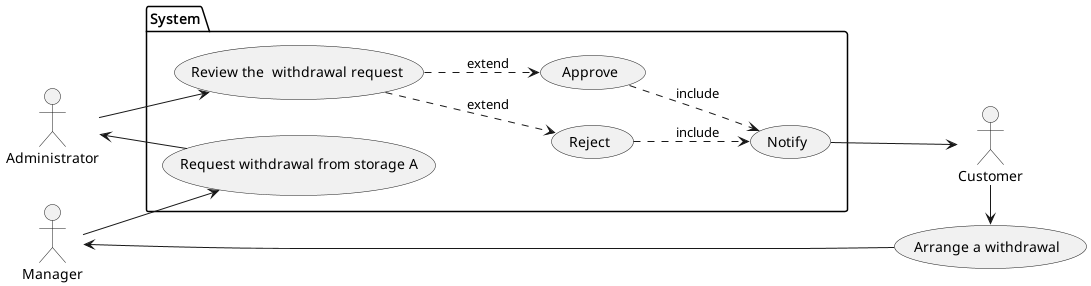
\includegraphics[width=12cm]{../../out/spec/figure/usecase/withdrawal_confirm/Storage Net, Use Case, Withdrawal.png}
  \caption{Use Case: Withdrawal}
\end{figure}

\subsection{Просмотр содержимого сети хранилищ}

\textbf{Участники:}
Менеджер.

\textbf{Описание:}
Менеджер может посмотреть содержимое заданного хранилища.
Еще менеджер может посмотреть содержимое всей сети.
Менеджер может посмотреть местонахождение предметов из заказа.

\begin{figure}[h]
  \centering
  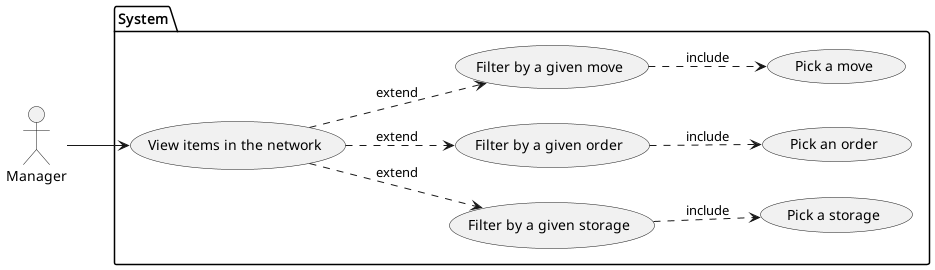
\includegraphics[width=12cm]{../../out/spec/figure/usecase/view/Storage Net, Use Case, View Content.png}
  \caption{Use Case: View}
\end{figure}

\section{Архитектура решения}

\subsection{Enity-Relationship Модель}

\subsubsection{Сущности}

\begin{enumerate}
  \item \textbf{Пользователь}: 
        идентификатор в HR системе, 
        ФИО.

  \item \textbf{Менеджер}: 
        является Пользователем, 
        связывается с заявками на перемещение,
        поставку и изъятие.

  \item \textbf{Администратор}:
        является Пользователем,
        управляет хранилищем,
        связывается с запросами на перемещение,
        поставку и изъятие,
        связывается с фактами поставки и изъятия.

  \item \textbf{Перевозчик}:
        note: отдельные таблицы для каждого,
        название перевозчика.

  \item \textbf{Заказчик}
        note: отдельные таблицы для каждого,
        название заказчика.

  \item \textbf{Хранилище}:
        содержит ячейки для хранения предметов,
        связано с Администратором,
        связано с операциями с ним.

  \item \textbf{Ячейка хранения}:
        хранилище в котором находится,
        хранит предметы одного типа,
        имеет тип хранимого предмета,
        имеет вместимость хранимых предметов.

  \item \textbf{Тип предмета}:
        имеет название,
        срок годности,
        единицы измерения 
        и прочую информацию.

  \item \textbf{INLINE Группа предметов}:
        идентификатор,
        тип предмета,
        количество > 0,
        дата изготовления,
        может быть заказ.

  \item \textbf{Перемещение}:
        идентификатор поездки у перевозчика,
        идентификатор перевозчика,
        дата отправления,
        дата прибытия,
        группы предметов,
        заявка на отправление,
        заявка на прибытие.

  \item \textbf{Заказ}
        заказчик,
        дата создания,
        дедлайн,
        связывается с перемещениями,
        связывается с изъятиями,
        мб связывается с поставками.

  \item \textbf{Поставка}
        поставщик,
        заявка на поставку,
        группы предметов.

  \item \textbf{INLINE Заявка в хранилище}
        хранилище,
        инициатор Менеджер,
        обработчик Администратор,
        принято в обработку,
        выполнено,
        дополнительная информация.

  \item \textbf{Изъятие}
        заказчик,
        заказ,
        заявка на изъятие,
        группы предметов.
  
  \item \textbf{Бронирование}
        заявка на бронирование,
        группа предметов,
        дата начала,
        дата снятия.

\end{enumerate}

\newpage

\subsubsection{Высокоуровневая ER-диаграмма}

\begin{figure}[h!]
      \centering
      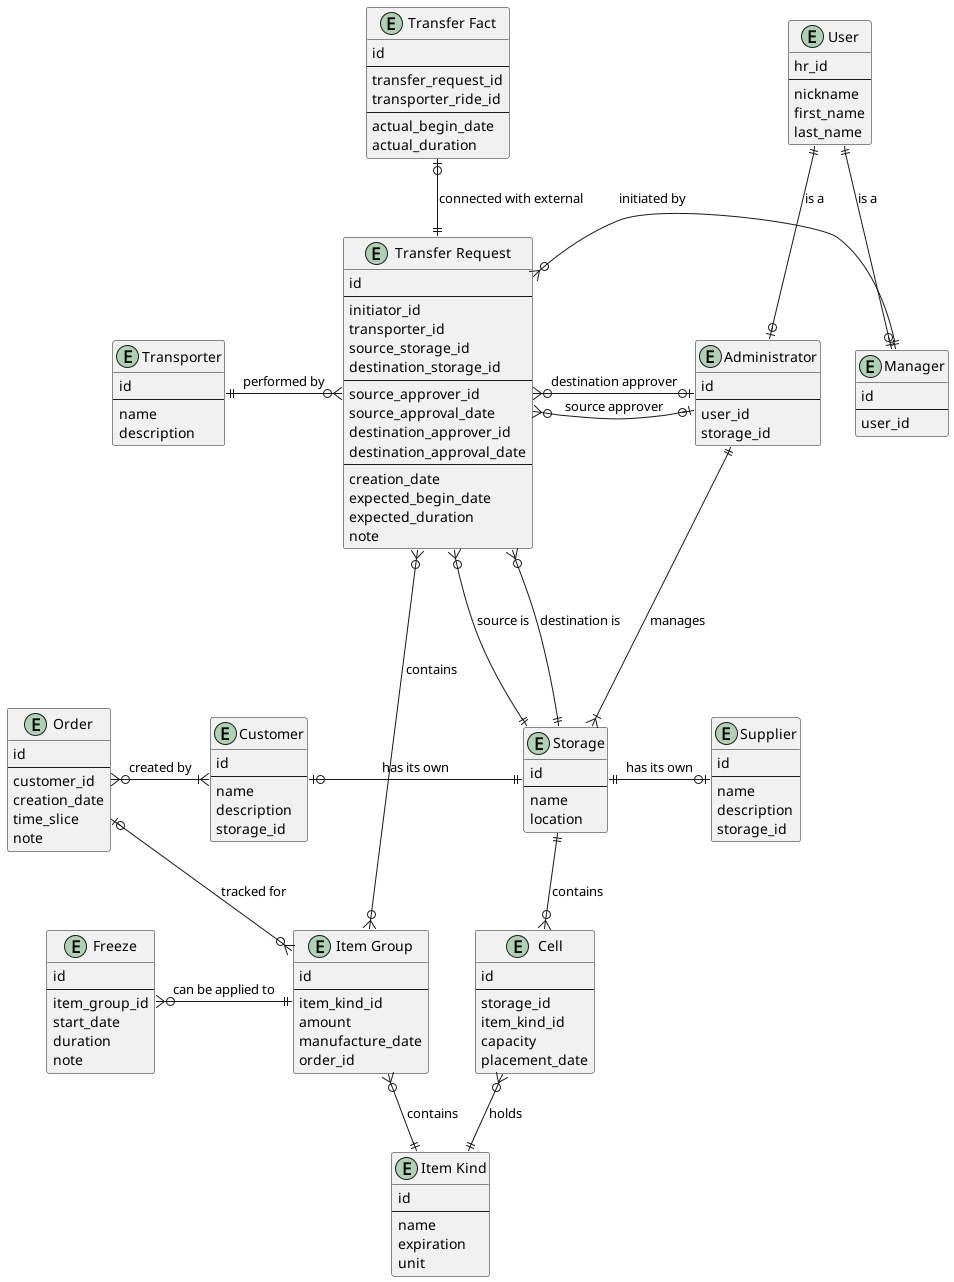
\includegraphics[width=12cm]{../../doc/spec/figure/er/high-level/Storage Net high-level ER Diagram.png}
      \caption{High-Level ER-Diagram}
\end{figure}

\newpage

\subsubsection{Низкоуровневая ER-диаграмма}

\begin{figure}[h!]
      \centering
      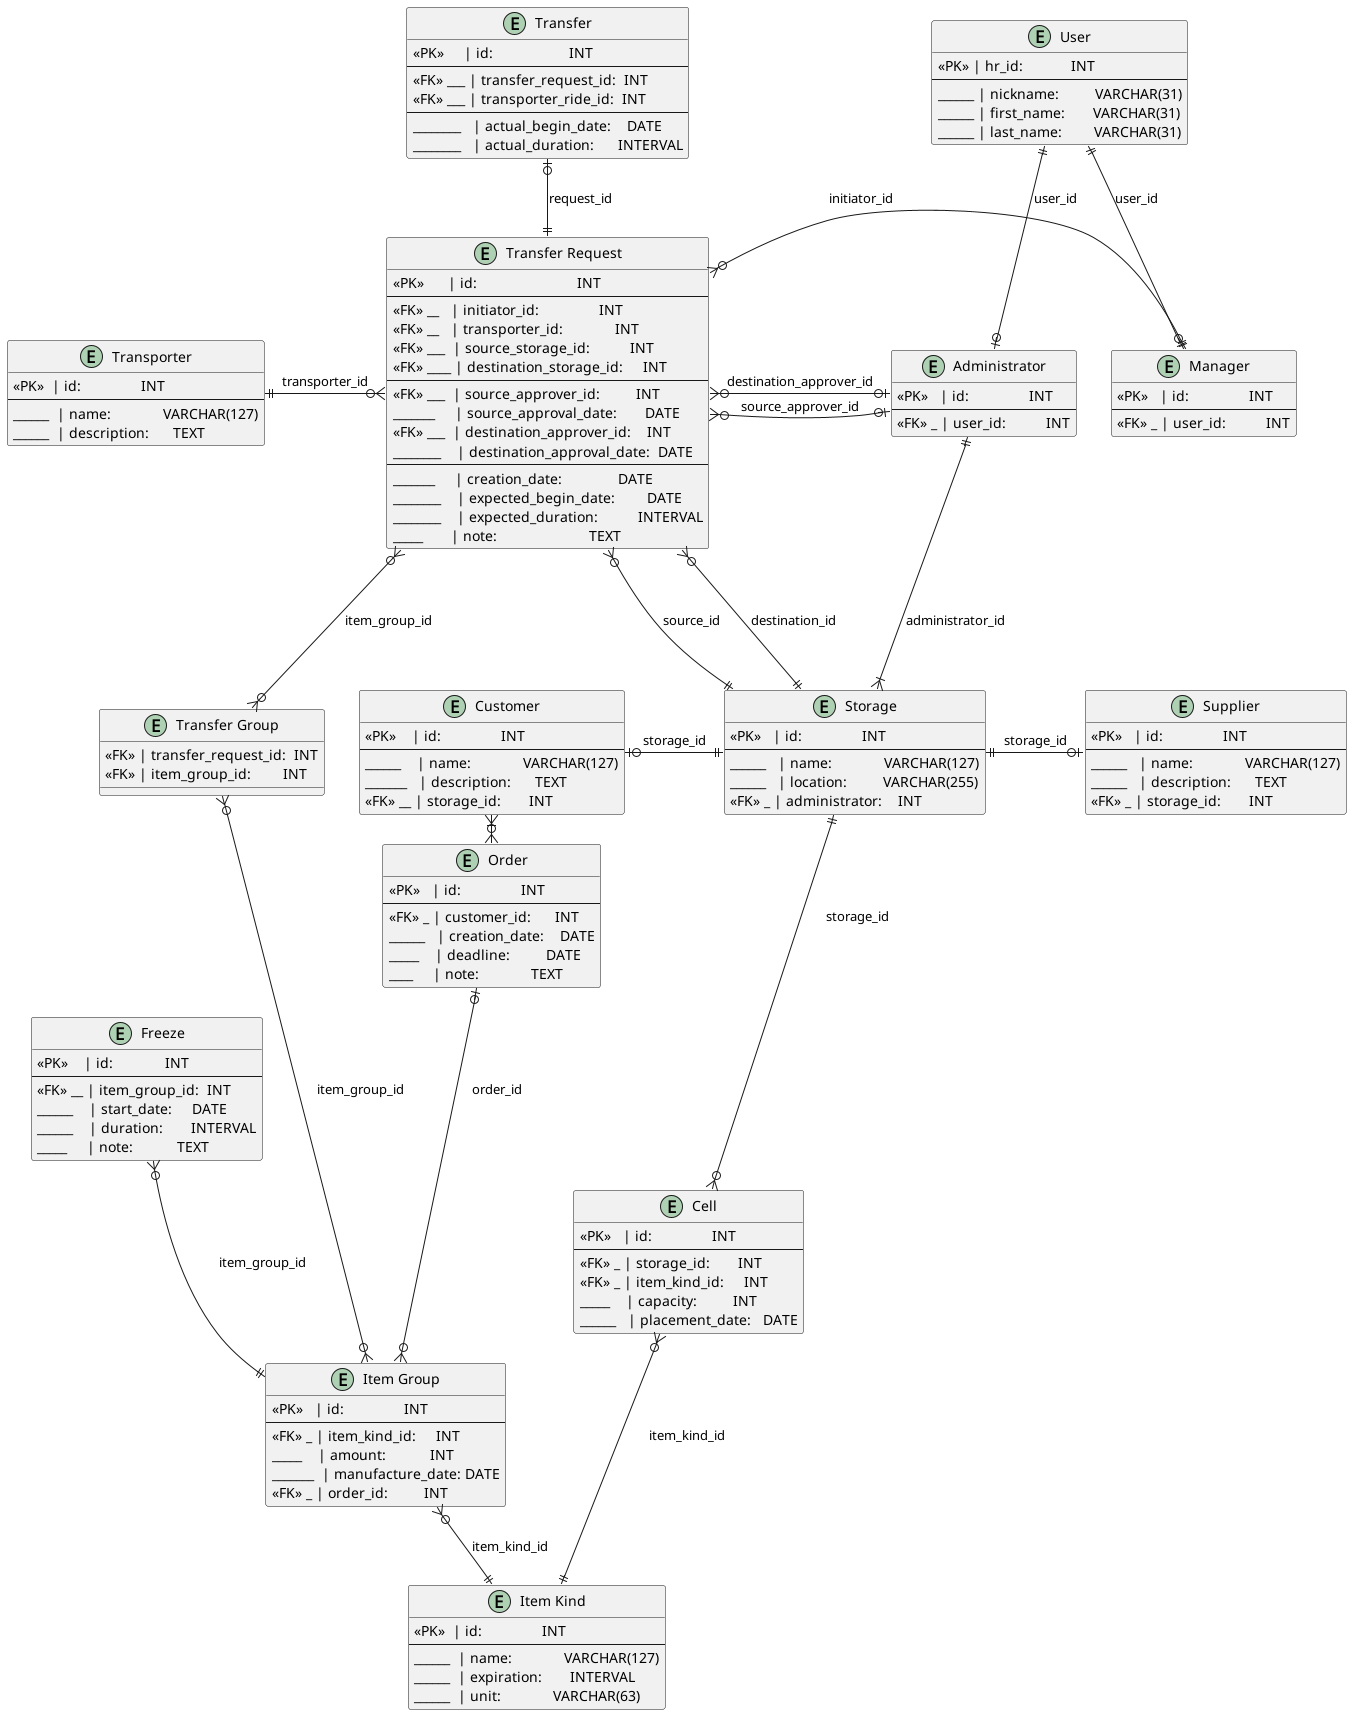
\includegraphics[width=12cm]{../../doc/spec/figure/er/low-level/Storage Net low-level ER Diagram.png}
      \caption{Low-Level ER-Diagram}
\end{figure}

\newpage


\end{document}